\documentclass{standalone}
\usepackage{tkz-euclide}
\usetkzobj{all} % Esta linha poderá ter que ser eliminada dependendo da versão do mikTex ou texLive

\begin{document}
	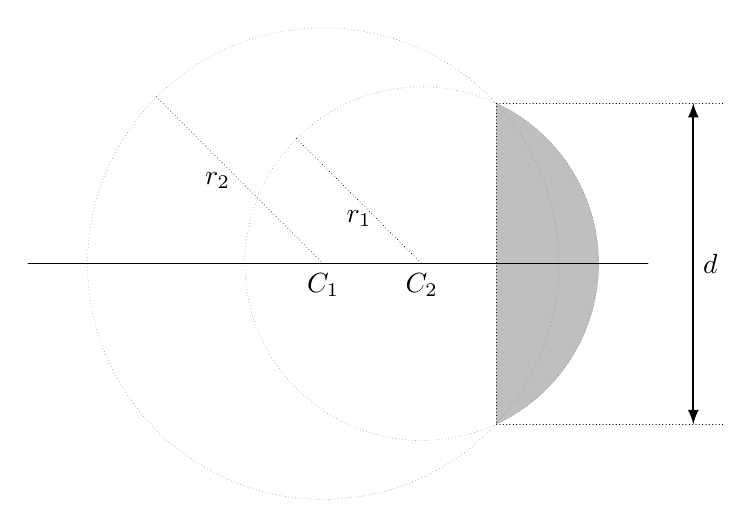
\begin{tikzpicture}
	\tkzDefPoints{0/0/C1, 1.25/0/C2}
	\tkzDefPoint(135:3){P1}
	\tkzDefPoint(135:2.25){P'2}
	\tkzDefPointBy[translation = from C1 to C2](P'2)\tkzGetPoint{P2}
	
	\tkzInterCC(C1,P1)(C2,P2)\tkzGetPoints{A1}{A2}
	\tkzDefPointBy[translation= from C1 to C2](A1)\tkzGetPoint{B1}
	\tkzDefPointBy[homothety=center A1 ratio 2](B1)\tkzGetPoint{D1}
	\tkzDefPointBy[translation= from C1 to C2](A2)\tkzGetPoint{B2}
	\tkzDefPointBy[homothety=center A2 ratio 2](B2)\tkzGetPoint{D2}
	
	\tkzDrawArc[fill=gray!50, draw=none](C2,A2)(A1)
		
	\tkzDrawCircle[densely dotted](C1,P1)
	\tkzDrawCircle[densely dotted](C2,P2)
	
	\tkzDrawSegment[densely dotted](A1,A2)
	\tkzDrawLine[densely dotted, add=0 and .15](A1,D1)
	\tkzDrawLine[densely dotted, add=0 and .15](A2,D2)
	\tkzDrawSegments[densely dotted](P1,C1 P2,C2)
	
	\tkzDrawSegment[thick, <->, >=latex](D1,D2)
	\tkzDrawLine[add = 3 and 2.3](C1,C2)
	
	\tkzLabelSegment[left](C1,P1){\(r_2\)}
	\tkzLabelSegment(C2,P2){\(r_1\)}
	\tkzLabelSegment[right](D1,D2){\(d\)}
	\tkzLabelPoint[below](C1){\(C_1\)}
	\tkzLabelPoint[below](C2){\(C_2\)}
	\end{tikzpicture}
\end{document}